\vspace*{6cm}
\lettrine[lines=1]{\color{redxlim}L}{oren} \gls{5g} psum dolor sit amet, consectetuer adipiscing elit. Ut purus elit, vestibulum ut, placerat ac, adipiscing vitae, felis. Curabitur dictum gravida mauris. Nam arcu libero, nonummy eget, consectetuer id, vulputate a, magna. Donec vehicula augue eu neque. Pellentesque habitant morbi tristique senectus et netus et malesuada fames ac turpis egestas. Mauris ut leo. Cras viverra metus rhoncus sem. Nulla et lectus vestibulum urna fringilla ultrices. Phasellus eu tellus sit amet tortor gravida placerat. Integer sapien est, iaculis in, pretium quis, viverra ac, nunc. Praesent eget sem vel leo ultrices bibendum. Aenean faucibus. Morbi dolor nulla, malesuada eu, pulvinar at, mollis ac, nulla. Curabitur auctor semper nulla. Donec varius orci eget risus. Duis nibh mi, congue eu, accumsan eleifend, sagittis quis, diam. Duis eget orci sit amet orci dignissim rutrum.~\cite{Osseiran2014}, \cite{Iwamura2015}, \cite{Evaluation2016} and \cite{Vu2017}:
\begin{enumerate}[nolistsep]
\item Data rates of tens of megabits per second for tens of thousands of users;
\item Data rates of 100 megabits per second for metropolitan areas;
\item 1 Gbps simultaneously to many workers on the same office floor;
\item Several hundreds of thousands of simultaneous connections for wireless sensors;
\item Spectral efficiency significantly enhanced compared to \gls{4g};
\item Coverage improved;
\item Signaling efficiency enhanced.
\end{enumerate}

\section{Examples}
\lipsum[1]

\begin{figure}[h]
	\centering
	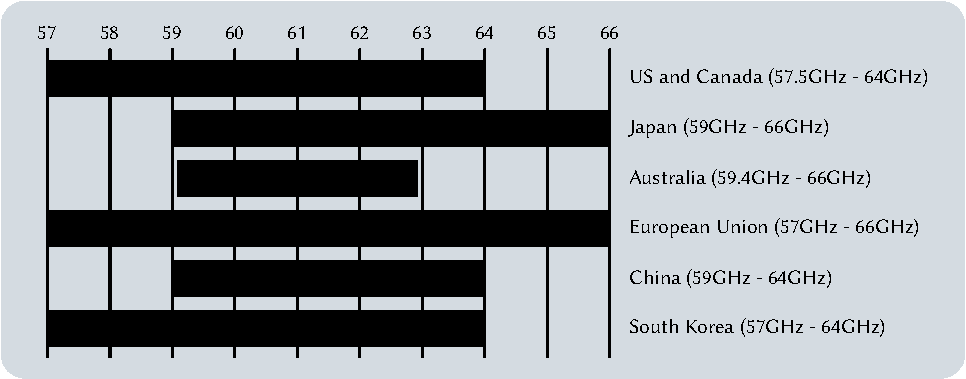
\includegraphics[width=0.8\textwidth]{chapters/images/ISM-60ghzBandAlocation}
		\caption{Example de figure}
		\label{fig-ISM60ghz}
\end{figure}

\lipsum[2]

\begin{table}
\centering
\caption{Example de tableau.}% Adapted from~\cite{Gupta2015}.}
\label{tab-evolution_mobile_network}
\tabulinesep=4pt
% \renewcommand{\arraystretch}{1.2}
\scalebox{0.8}{%
\begin{tabu}to 1.25\textwidth{X[l,m]m{70pt}m{85pt}m{60pt}m{70pt}m{40pt}m{50pt}m{60pt}}
\toprule
\tableHeaderStyle
%-------------------------
	Gen								& 
	Access Tech.					&
	Data Rate						& 
	Freq. Band						& 
	BW								&
	Error Coding					& 
	Switching						& 
	Applications					\\
	\midrule
%-------------------------
	1G								    & 
	\makecell[l]{\gls{amps}\\\gls{fdma}}& 
	2.4 kbps							& 
	800 MHz								& 
	30 kHz								& 
	NA								    &
	Circuit								& 
	Voice								\\
	\midrule
%-------------------------
									    & 
	\makecell[l]{\gls{gsm}\\\gls{tdma}}	&
	10 kbps								& 
	\cellcolor[gray]{0.9}				& 
	200 kHz								& 
	\cellcolor[gray]{0.9}				& 
									    & 
	\cellcolor[gray]{0.9}				\\
	\cmidrule{2-3}\rulefiller{4-4}\cmidrule{5-5}\rulefiller{6-6}\rulefiller{8-8}
%-------------------------
	\multirowcell{-2}[0pt][l]{2G}	    & 
	\gls{cdma}						    & 
	10 kbps							    & 
	\cellcolor[gray]{0.9}			    & 
	1.25 MHz						    & 
	\cellcolor[gray]{0.9}				& 
	\multirowcell{-2}[6pt][l]{Circuit}	&
	\cellcolor[gray]{0.9}				\\
	\cmidrule{1-3}\rulefiller{4-4}\cmidrule{5-5}\rulefiller{6-6}\cmidrule{7-7}\rulefiller{8-8}
%-------------------------
							& 
	\gls{gprs}				& 
	50 kbps					& 
	\cellcolor[gray]{0.9}	& 
	200 kHz					& 
	\cellcolor[gray]{0.9}	& 
							& 
	\cellcolor[gray]{0.9}						\\
	\cmidrule{2-3}\rulefiller{4-4}\cmidrule{5-5}\rulefiller{6-6}\rulefiller{8-8}
%-------------------------
	\multirowcell{-2}[0pt][l]{2.5G}	                                			& 
	\gls{edge}								                                    & 
	200 kbps							                                        & 
	\cellcolor[gray]{0.9}\multirowcell{-4}[6pt][l]{850/\\900/\\1800/\\1900 MHz}	&
	200 kHz								                                        & 
	\cellcolor[gray]{0.9}\multirowcell{-4}[6pt][l]{NA}					        & 
	\multirowcell{-2}[-4pt][l]{Circuit,\\Packet}			                    &
	\cellcolor[gray]{0.9}\multirowcell{-4}[6pt][l]{Voice,\\Data}	            \\
	\midrule
%-------------------------
									        & 
	\makecell[l]{\gls{wcdma}\\\gls{umts}}	&	 
	384 kbps							    & 
	\cellcolor[gray]{0.9}					& 
	5 MHz								    & 
	\cellcolor[gray]{0.9} 					& 
								        	& 
	\cellcolor[gray]{0.9} 					\\
	\cmidrule{2-3}\rulefiller{4-4}\cmidrule{5-5}\rulefiller{6-6}\rulefiller{8-8}
%-------------------------
	\multirowcell{-2}[0pt][l]{3G}				& 
	\gls{cdma2k}							    & 
	384 kbps							        & 
	\cellcolor[gray]{0.9}						& 
	1.25MHz							        	& 
	\cellcolor[gray]{0.9}						& 
	\multirowcell{-2}[8pt][l]{Circuit,\\Packet}	& 
	\cellcolor[gray]{0.9}						\\
	\cmidrule{1-3}\rulefiller{4-4}\cmidrule{5-5}\rulefiller{6-6}\cmidrule{7-7}\rulefiller{8-8}
%-------------------------
									        & 
	\makecell[l]{\gls{hsupa}\\\gls{hspda}}  & 
	5--30 Mbps							    & 
	\cellcolor[gray]{0.9} 					& 
	5 MHz								    & 
	\cellcolor[gray]{0.9} 					& 
									        & 
	\cellcolor[gray]{0.9} 					\\
	\cmidrule{2-3}\rulefiller{4-4}\cmidrule{5-5}\rulefiller{6-6}\rulefiller{8-8}
%-------------------------
	\multirowcell{-2}[0pt][l]{3.5G}			                                    		& 
	\gls{evdo}								                                            & 
	5--30 Mbps					                                                        & 
	\cellcolor[gray]{0.9}\multirowcell{-4}[18pt][l]{800/\\850/\\900/\\1800/\\2100MHz}	& 
	1.25 MHz							                                                & 
	\cellcolor[gray]{0.9}\multirowcell{-4}[18pt][l]{Turbo\\Codes}				        & 
	\multirowcell{-2}[8pt][l]{Packet}				                                    & 
	\cellcolor[gray]{0.9}\multirowcell{-4}[18pt][l]{Voice,\\Data,\\Video\\calling}	    \\
	\midrule
%-------------------------
									                    & 
	\makecell[l]{\gls{lte}\\\gls{ofdma}/\\\gls{scfdma}}	& 
	\makecell[l]{100--200 Mbps}					        & 
	\makecell[l]{1.8,\\2.6~GHz}					        & 
	\makecell[l]{1.4 -- 20 MHz}					        & 
	\cellcolor[gray]{0.9}						        & 
	\cellcolor[gray]{0.9}						        & 
	\cellcolor[gray]{0.9}						        \\
	\cmidrule{2-5}\rulefiller{6-6}\rulefiller{7-7}\rulefiller{8-8}
%-------------------------
	\multirowcell{-2}[0pt][l]{3.75G}				                            & 
	\makecell[l]{\gls{wimax}\\\gls{sofdma}}					                    & 
	\makecell{100--200 Mbps}					                                & 
	\makecell[l]{3.5,\\5.8 GHz\\(initially)}			                        & 
	1.25 MHz							                                        & 
	\cellcolor[gray]{0.9}\multirowcell{-2}[-3pt][l]{Concat.\\Codes}			    & 
	\cellcolor[gray]{0.9}\multirowcell{-2}[-3pt][l]{Packet}			        	& 
	\cellcolor[gray]{0.9}\multirowcell{-2}[-3pt][l]{Online\\gaming,\\\gls{hdtv}}\\
	\midrule
%-------------------------
									                    & 
	\makecell[l]{\gls{ltea}\\\gls{ofdma}/\\\gls{scfdma}}& 
	\parbox{76pt}{DL~3~Gbps\\UL~1.5~Gbps}				& 
	\makecell[l]{1.8,\\2.6 GHz}					        & 
	\makecell[l]{1.4--20 MHz}					        & 
	\cellcolor[gray]{0.9}						        & 
	\cellcolor[gray]{0.9}						        & 
	\cellcolor[gray]{0.9}						        \\
	\cmidrule{2-5}\rulefiller{6-6}\rulefiller{7-7}\rulefiller{8-8}
%-------------------------
	\multirowcell{-2}[0pt][l]{4G}					                            & 
	\makecell[l]{\gls{wimax}\\(Mobile)\\\gls{sofdma}}				            & 
	\makecell[l]{100--200 Mbps}					                                & 
	\makecell[l]{2.3, 2.5 and\\3.5 GHz\\(initially)}		                    & 
	\makecell[l]{3.5, 7,\\5, 10 and\\8.75 MHz\\(initially)}		                & 
	\cellcolor[gray]{0.9}\multirowcell{-2}[-3pt][l]{Turbo\\Codes}				& 
	\cellcolor[gray]{0.9}\multirowcell{-2}[-3pt][l]{Packet}				        & 
	\cellcolor[gray]{0.9}\multirowcell{-2}[-3pt][l]{Online\\gaming,\\\gls{hdtv}}\\
	\midrule
%-------------------------
	5G								                            & 
	\makecell[l]{\gls{bdma}\\\gls{fbmc}}					    &
	\makecell[l]{10--50 Gbps\\(expected)}				        & 
	\makecell[l]{1.8,\\ 2.6 GHz and\\\gls{mmwaves}\\(expected)}	& 
	will depend on the quantity of channels in use				& 
	\gls{ldpc}								                    & 
	Packet								                        & 
	\makecell[l]{\gls{uhdtv}\\Video,\\\gls{vr} app.}			\\
\bottomrule
\end{tabu}}
% \vspace{-4pt}
\begin{tablenotes}
\small
\item \hfill * Table adapted from~\cite{Gupta2015}
\end{tablenotes}
\end{table}
